\section{Atividade 1}
\subsection{Descrição do Modelo}
O sistema modelado é um oscilador massa-mola-amortecedor, onde a massa está sujeita à força restauradora de uma mola e ao amortecimento proporcional à velocidade. A equação diferencial que descreve o movimento do sistema é dada por:
\[
    m \ddot{x} + C \dot{x} + Kx = 0
\]
onde \( x \) representa o deslocamento da massa \( m \) da sua posição de equilíbrio, \( \dot{x} \) é a velocidade, \( \ddot{x} \) é a aceleração, \( C \) é o coeficiente de amortecimento, e \( K \) é a constante da mola. A força de entrada é considerada nula, indicando que não há forças externas atuando sobre o sistema após o instante inicial.

\subsection{Parâmetros do Sistema}
Os parâmetros utilizados no modelo do sistema são especificados como segue:
\begin{itemize}
    \item Massa (\( m \)): 10 kg
    \item Coeficiente de amortecimento (\( C \)): 7 Ns/m
    \item Constante da mola (\( K \)): 5 N/m
\end{itemize}

\subsection{Condições Iniciais para a Simulação}
As condições iniciais para a simulação são detalhadas na tabela a seguir, baseadas nos parâmetros especificados acima:
\begin{center}
    \begin{tabular}{|c|c|c|}
        \hline
        \textbf{Caso} & \textbf{Velocidade Inicial \( V_0 \)} & \textbf{Posição Inicial \( X_0 \)} \\
        \hline
        1             & \( 5 \, \text{m/s} \)                 & \( 0 \, \text{m} \)                \\
        2             & \( 0 \, \text{m/s} \)                 & \( 2.5 \, \text{m} \)              \\
        3             & \( 3.33 \, \text{m/s} \)              & \( 2 \, \text{m} \)                \\
        \hline
    \end{tabular}
\end{center}

Esta tabela reflete os valores numéricos para cada caso, facilitando a compreensão e a aplicação direta dos parâmetros na simulação.

\subsection{Análise dos Resultados}
Cada um dos casos de simulação foi configurado com condições iniciais distintas para explorar como o sistema responde a diferentes estados iniciais de deslocamento e velocidade.

\subsubsection{Caso 1: Velocidade Inicial Elevada}
\begin{figure}[H]
    \centering
    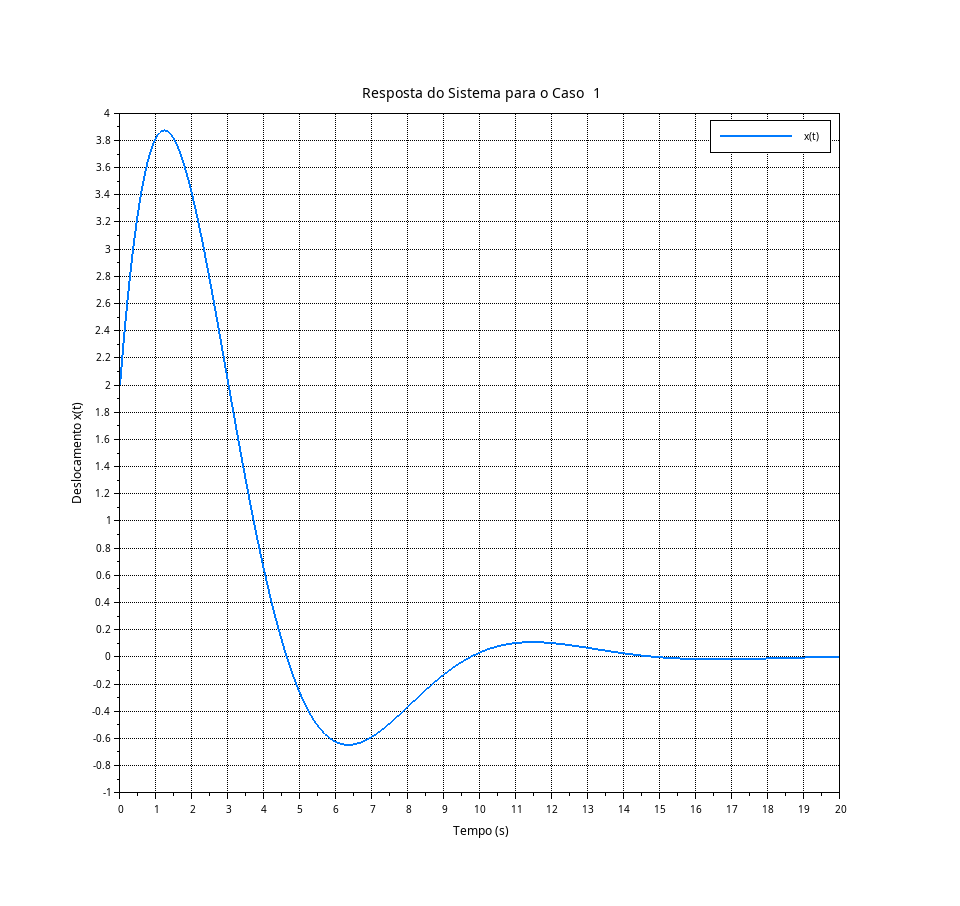
\includegraphics[width=0.6\textwidth]{final/1-atividade/assets/caso1.png}
    \caption{Resposta do sistema para o Caso 1}
\end{figure}
No Caso 1, o sistema é inicialmente impulsionado com uma alta velocidade (\(5 \, \text{m/s}\)), partindo do repouso (\(X_0 = 0\)). Esta condição inicial leva a uma resposta inicialmente enérgica, onde a massa oscila com uma amplitude elevada, seguida de um rápido decaimento energético devido ao amortecimento significativo (\(C = 7 \, \text{Ns/m}\)). O amortecimento não só reduz a amplitude das oscilações rapidamente, mas também garante que o sistema não persista em um estado de oscilação prolongada, estabilizando-se em um tempo curto.

\subsubsection{Caso 2: Deslocamento Inicial Sem Velocidade}
\begin{figure}[H]
    \centering
    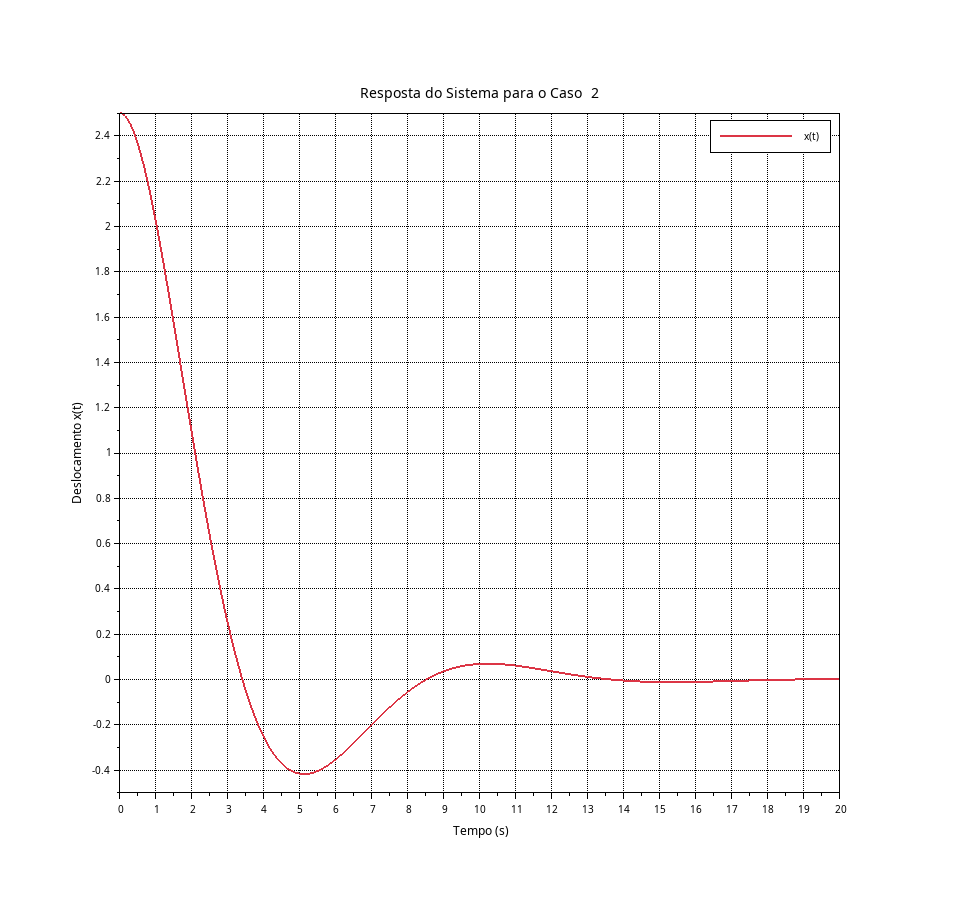
\includegraphics[width=0.6\textwidth]{final/1-atividade/assets/caso2.png}
    \caption{Resposta do sistema para o Caso 2}
\end{figure}
O Caso 2 é caracterizado por um deslocamento inicial (\(2.5 \, \text{m}\)) sem impulso inicial de velocidade (\(V_0 = 0\)). Aqui, observamos uma resposta típica de um sistema oscilatório subamortecido onde o sistema retorna ao equilíbrio através de oscilações que decaem gradativamente. Este caso destaca como a energia potencial armazenada na mola é convertida em energia cinética e dissipada pelo amortecedor. As oscilações decrescem em amplitude mais gradualmente do que no Caso 1, demonstrando uma transferência de energia mais prolongada antes da estabilização.

\subsubsection{Caso 3: Velocidade e Deslocamento Iniciais}
\begin{figure}[H]
    \centering
    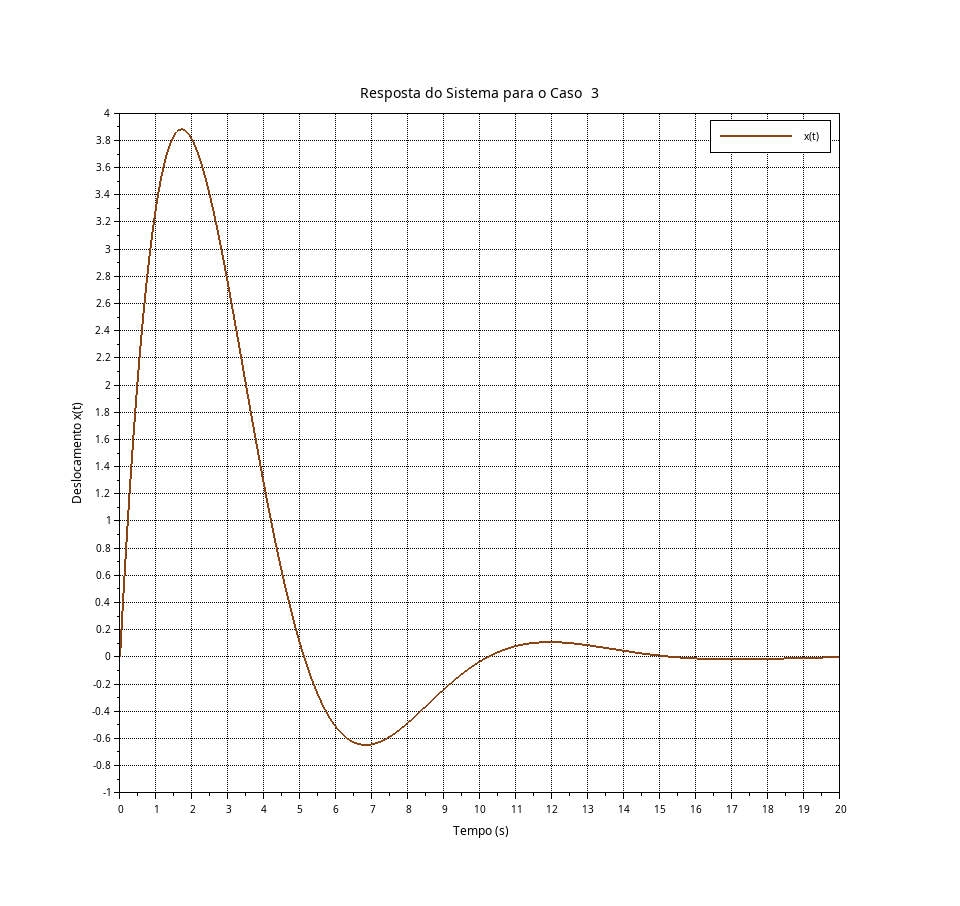
\includegraphics[width=0.6\textwidth]{final/1-atividade/assets/caso3.png}
    \caption{Resposta do sistema para o Caso 3}
\end{figure}
No Caso 3, o sistema inicia com condições iniciais moderadas tanto de velocidade (\(3.33 \, \text{m/s}\)) quanto de deslocamento (\(2 \, \text{m}\)). Esta configuração produz uma resposta dinâmica complexa, onde a interação entre energia cinética e potencial é mais evidente. A amplitude inicial é significativa, com uma taxa de decaimento que ilustra eficientemente o papel do amortecimento. As oscilações observadas são mais sustentadas que no Caso 1, mas menos intensas do que no Caso 2, refletindo um equilíbrio entre as energias cinética e potencial no início da simulação.

\subsubsection{Comparação Unificada dos Casos}
\begin{figure}[H]
    \centering
    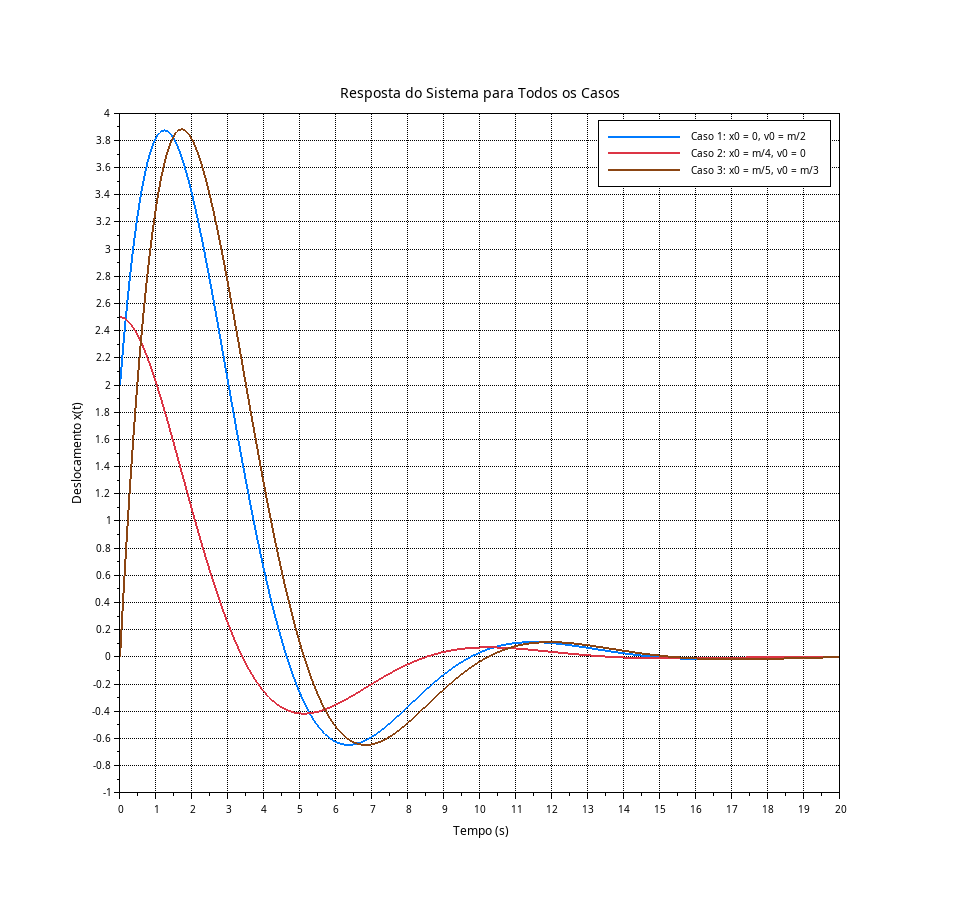
\includegraphics[width=0.6\textwidth]{final/1-atividade/assets/caso-all-in-one.png}
    \caption{Resposta unificada do sistema para os Casos 1, 2 e 3}
\end{figure}
A análise unificada dos três casos demonstra de forma clara as diferenças significativas nas respostas do sistema decorrentes de diversas condições iniciais. A seguir, discutiremos detalhadamente cada resposta e suas implicações para a compreensão do comportamento dinâmico do sistema:

\begin{itemize}
    \item \textbf{Caso 1 (Azul Escuro)}: Iniciado com uma alta velocidade inicial (\(5 \, \text{m/s}\)) e sem deslocamento inicial, este caso exibe a maior amplitude de oscilação observada. A energia cinética inicial é rapidamente convertida em energia potencial pela mola, resultando em oscilações de grande amplitude que são rapidamente amortecidas. Este caso ilustra o efeito de um forte amortecimento, onde a energia é dissipada rapidamente, levando a um retorno rápido à posição de equilíbrio sem oscilações residuais prolongadas. Esta configuração é ideal em situações onde a rápida estabilização após distúrbios é crucial, como em sistemas de suspensão de veículos.

    \item \textbf{Caso 2 (Vermelho)}: Com um deslocamento inicial (\(2.5 \, \text{m}\)) e sem velocidade inicial, o sistema mostra uma resposta clássica de um oscilador subamortecido. A energia potencial armazenada na mola é convertida gradualmente em energia cinética, com a energia sendo dissipada ao longo do tempo pelo amortecedor. As oscilações decaem suavemente, refletindo uma conversão mais lenta de energia que é típica em aplicações onde é necessário manter uma certa quantidade de movimento ou onde oscilações graduais são preferíveis, como em alguns tipos de sensores mecânicos.

    \item \textbf{Caso 3 (Marrom)}: Este caso combina condições iniciais moderadas de velocidade (\(3.33 \, \text{m/s}\)) e deslocamento (\(2 \, \text{m}\)), resultando numa resposta dinâmica mais complexa que engloba características dos dois primeiros casos. A amplitude inicial é significativa, mas as oscilações são mais controladas e decaem de maneira gradual. Este caso destaca a importância do equilíbrio entre rigidez da mola e amortecimento no projeto de sistemas mecânicos, onde é necessário um compromisso entre estabilidade rápida e manutenção de energia dinâmica.
\end{itemize}

Esta comparação detalhada destaca não apenas a influência das condições iniciais na resposta do sistema, mas também o papel crítico do amortecimento e da rigidez da mola na determinação da natureza da resposta dinâmica. A análise fornece insights valiosos para o design e a otimização de sistemas mecânicos em engenharia, sublinhando a necessidade de uma seleção cuidadosa de parâmetros de acordo com os requisitos específicos de cada aplicação.


\subsection{Comentários Gerais e Conclusão}
Os gráficos e análises ilustram claramente como as condições iniciais impactam a resposta dinâmica do sistema massa-mola-amortecedor. A energia inicial, seja como deslocamento ou velocidade, define a resposta imediata do sistema, mostrando a complexidade do comportamento de sistemas dinâmicos lineares. Observamos que o amortecimento é essencial para reduzir as oscilações e trazer o sistema de volta ao repouso de maneira eficiente, sublinhando sua importância no design de componentes mecânicos.

A adequação do coeficiente de amortecimento e da rigidez da mola é crucial para otimizar sistemas para suas funções específicas, como a absorção de choques em suspensões de veículos ou a precisão em instrumentos de medição. Além disso, a análise das condições iniciais é vital no planejamento e teste de sistemas mecânicos, onde engenheiros e designers devem antecipar cenários variados de operação.

Este estudo destaca a necessidade de um entendimento profundo das dinâmicas de sistemas para inovação em engenharia, proporcionando uma base sólida para a compreensão dos princípios de mecânica e dinâmica que são fundamentais no design de sistemas controlados e mecanismos em geral.
